\documentclass[a4paper, 10pt, conference]{ieeeconf}

\usepackage{cite}
\usepackage{latexsym,amsfonts,amssymb,graphicx,amsmath}
\usepackage{url}
% Read the url.sty source comments for usage information. Basically,
% \url{my_url_here}.

% correct bad hyphenation here
\hyphenation{op-tical net-works semi-conduc-tor}
\bibliographystyle{./IEEEtran}
\IEEEoverridecommandlockouts

\title{\LARGE \bf
A low cost, scalable, \\ virtual control laboratory
}

\author{Inderpreet Arora, Kannan M. Moudgalya, Kaushik Venkata, Victor
  Chakraborty, Rupak Rokade and Rakhi R.%
\thanks{Inderpreet Arora is a former student of Systems and Control
  Engineering, IIT Bombay, Mumbai, India. She is currently with the
  Eaton India Engineering Center, Eaton Corporation, Pune, India. 
        {\tt\small inderpreet.arora@iitb.ac.in}}
\thanks{Kannan M. Moudgalya is a Core Faculty member with Department
  of Chemical Engineering and an Associate Faculty member with Systems
  and Control Engineering, IIT Bombay, Mumbai, India. 
        {\tt\small kannan@iitb.ac.in}}%
\thanks{Kaushik Venkata is a student of Systems and Control
  Engineering, IIT Bombay, Mumbai, India. 
        {\tt\small kaushik8989@iitb.ac.in}}
\thanks{Victor Chakrabory is a student of Department of Computer
  Science Engineering, IIT Bombay, Mumbai, India. 
        {\tt\small victor@cse.iitb.ac.in}}
\thanks{Rupak Rokade and Rakhi R. are Research Associates with
  Department of Chemical Engineering, IIT Bombay, Mumbai, India. 
        {\tt\small rupakrokade@iitb.ac.in, rakhi@iitb.ac.in}}%
}
%

\newcommand{\figref}[1]{Fig.~\ref{#1}}
\begin{document}

\maketitle
\thispagestyle{empty}
\pagestyle{empty}


\begin{abstract}
  This work presents a virtual control laboratory, based on a single
  board heater system and free and open source software, such as
  Scilab, Xcos, Java, PHP/MySQL and GNU/Linux.  This solution allows
  of the order of 20 devices to be handled by a single Server PC.  It
  allows many students to carry out control experiments remotely.
  It has been extensively tested
  in two control courses at IIT Bombay.  Results of a few experiments,
  conducted remotely, using this setup are presented.
\end{abstract}

\section{Introduction}
\label{sec:intro}
The objective of this work is to provide control laboratory
education to students who may not have access to good infrastructure.
This can be further detailed into the following specific objectives:
\begin{enumerate}
\item Provide a low cost laboratory.  One should be able to create,
  operate and maintain the laboratory at a low cost.  This requirement
  can be further divided into two sub-requirements:
\begin{enumerate}
\item Low cost hardware
\item Free software
\end{enumerate}
\item Provide remote access so that only Internet access is required
  at the student end.
\item Provide good learning experience:  It is not enough if the
  students enter parameters of a control algorithm, for example, P, I,
  D parameters;  they should be able to develop and validate their own
  control algorithm.
\item Scale the solution so that a large number of students can access
  the laboratory facility simultaneously.  This is important in the
  Indian context that has about a million students enrolling in
  engineering studies every year.
\item Access to a large number of students should be made with minimal
  infrastructure.  For example, the computer server and the Internet
  Protocol (IP) address should be able to accommodate many apparatus
  simultaneously.  This will allow minimally endowed Centres also to
  replicate such a facility and thus help evolve a distributed
  solution.  
\end{enumerate}
The issues raised in points 1(a) and 2 have been addressed in
\cite{ia010,vlabs-kmm} through a single board heater system (SBHS).
In the current work, we address all the remaining issues.  We begin
with a brief literature survey.  


% Hands-on experimentation is an important learning component for
% engineering education.  However, there is a lack of proper
% infrastructure, especially in remote areas, in India. Additionaly, the
% existing expensive lab equipments impose restrictions on type and
% duration of the experiments that could be done by the students.  This
% paper depicts a low cost single-board heater system virtual lab to
% address these issues. 

% Section 2 briefly discusses the features of the low cost, open source,
% single-board heater system (SBHS).  The low cost of a device is not
% enough to attract academia.  We explore the possibility of using this
% $\$50$ device as a part of virtual lab. 

% Though the web based labs have been in practice in a few countries for
% quite some time their usage in India is uncommon.  Section 3 explains
% the evolution of virtual labs for SBHS. Section 4 depicts the current
% hardware and software architecture of virtual SBHS lab at IIT Bombay.
% This lab allows the access of a single-board heater system, a control
% setup, through internet.  The control experiments performed on this
% setup, over internet, are described in Section 5. 

\section{Literature Survey}
\label{sec:litsurvey}
We now present a brief, non-exhaustive, survey of virtual laboratory
work reported in the last couple of years.


The work reported in \cite{carlos} allows multiple users the access to
experimental and computational resources through only a Web browser, a
low-bandwidth Internet connection, and low user-side technical
specifications.  The server side is scalable and reproducible since it
is based on Linux operating system.  This solution makes use of a
Matlab license.   

The work reported in
\cite{aldo} can be used as a portable telelaboratory, completely
contained inside a Live Linux-RTAI DVD, which can be connected to a
large number of real plant to perform a process supervision task. 
This lab architecture makes use of RTAI-Linux and COMEDI and
alogorithms could be implemented in Matlab or Scilab.  

The work reported in \cite{odeh} allows the student to connect
components and equipment such as capacitors, resistors, transistors,
function generators with a switch system of a lab server and to map it
to a configuration data structure.  At run time, the GUI gets
constructed automatically, using Adobe Flash CS3.

The work reported in \cite{gabriel} is based on a PLC and ATmega8
microcontroller for data acquisition and control.  
The PLC is programmed using OMRON CX programmer 5.0 and the
microcontroller is programmed through AVR Studio 4.0.  The software
component is based on Java and MySQL.  Live video is a part of this
solution. 

The work reported in \cite{alberto} provide remote access to a
thermal control plant and a velocity control plant.  The former is
built with off-the-shelf components (some transistors and temperature
sensors), whereas the latter uses standard LEGO elements and minimal
electronics.  This work makes use of LabVIEW.


\section{Single Board Heater System (SBHS)}
A single-board heater system is a low cost, open source, lab-in-a-box
setup \cite{ia010}.  It consists of a heater assembly, fan,
temperature sensor, ATmega16 microcontroller and associated
circuitry. A stainless steel blade whose temperature has to be
controlled serves as the plant.  Nichrome helical coil with 20 turns
kept at a small distance from the steel blade, acts as the heater
element.  AD590, a monolithic integrated circuit temperature
transducer, is soldered beneath the steel plate.  A computer fan, a
low cost and commercially off the shelf component, is used to cool the
plate from below.

The plant has a small time constant, less than a minute, that allows
completion of an experiment in a short time.  This in turn facilitates
performance of a large number of experiments in a single laboratory
session.  The speed of response not being too fast allows the
measurements to be seen with naked eye, as it happens in industrial
systems.  It also demonstrates other measurement issues, such as,
noise. 

The codes for hardware interface and control experiments, and manuals
are available at \cite{vl010,moodle}.  Unlike \cite{ia010}, for the
purpose of remote access, 252 until 255 are reserved as command words
where 252 is meant for communication of machine I.D. This allows fan
input to vary from 0 to 251 PWM (Pulse Width Modulation) units. 

\section{Evolution of SBHS virtual labs}
In \cite{vlabs-kmm}, 
the control algorithm is implemented at the server end and the remote
student just keys in the parameters, as shown in Figure
\ref{fig:initial}. 
\begin{figure}
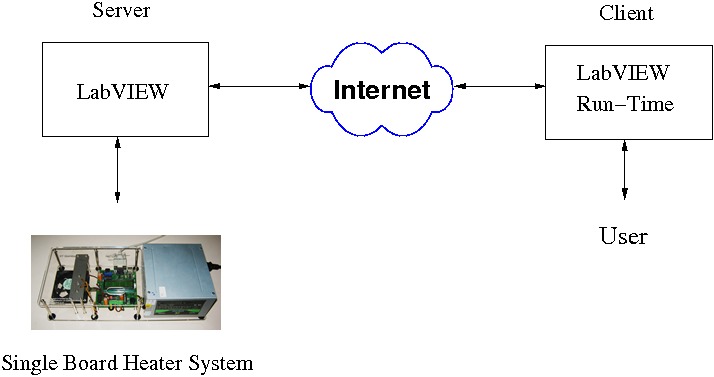
\includegraphics[width=\linewidth]{IEEE-Chile/figures/vlab-1.png}
\caption{SBHS virtual laboratory with remote access using LabVIEW}
\label{fig:initial}
\end{figure}
LabVIEW was used for the implementation of the same. The
server end consisted of a computer connected with an SBHS with a full
blown copy of LabVIEW installed on it. The client has a LabVIEW run
time engine available for free download from the National Instruments
website.  A few
LabVIEW algorithms/experiments were hosted on the server. The client
accesses these algorithm/experiment over the Internet using a web
browser by entering appropriate parameters.

It was realized that the learning experience is not complete for this
structure. This is because the server hosts some pre-built LabVIEW
algorithms and a user can only access these few algorithms. The user
can in no way change the program and can only input experimental
parameters. 
Hence, we came up with a new architecture
as shown in the Figure \ref{fig:second} that used full blown copies of
LabVIEW at both server and client ends.  
\begin{figure}
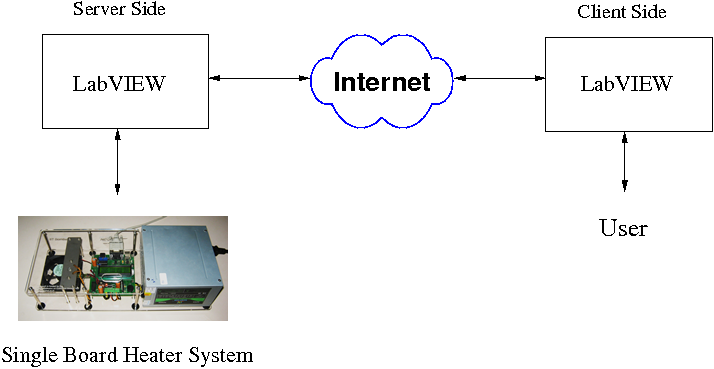
\includegraphics[width=\linewidth]{IEEE-Chile/figures/vlab-2.png}
\caption{SBHS virtual laboratory with remote access and live data sharing using LabVIEW}
\label{fig:second}
\end{figure}
 
 This idea uses the DataSocket technology of LabVIEW. Since now the
 client is having a complete LabVIEW installation on his/her computer
 she can now implement her own algorithms.  Thus this architecture did
 provide a complete learning experience to the students.  There are
 some shortcomings as well:

\begin{itemize}
\item LabVIEW is expensive and students may not be able to afford to
  buy it.  It is also prohibitively expensive for the Government to
  distribute it.

\item We used the LabVIEW version 8.04, which had restricted scripting
  language.  It was tedious to create new control algorithms in it.
\end{itemize}
\begin{figure}
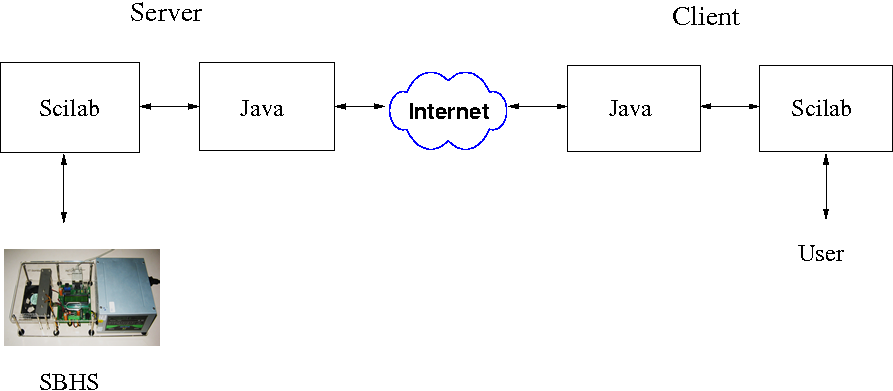
\includegraphics[width=\linewidth]{IEEE-Chile/figures/vlab-3.png}
\caption{SBHS virtual laboratory using open source software}
\label{fig:third}
\end{figure}
This made us shift to free and open source (FOSS) software. We
replaced LabVIEW with Java and Scilab as shown in Figure
\ref{fig:third}. Scilab at the server end is used for communicating
with SBHS. Scilab at the client end is used for implementing the
algorithms. Java is used at both the server as well as client end for
communication over the Internet thereby connecting the client with the
server. 

For the above solution, we need a dedicated copy of scilab running at
the server end for every SBHS. One way to do this is to host it on
multiple computers with unique IPs. Hence the number of SBHS we want
to host requires as many computer's and public IPs thereby making
it expensive. Moreover, it also limits its scalability. The other way
to do this is to host multiple java and scilab servers on the same
computer.  Hosting many copies of Scilab simultaneously requires a
powerful computer for the server.

For these reasons  we decided to take scilab off the server computer
and to use java alone to communicate with the SBHS directly.  Java
also 
communicates with the client computer.  We connected seven SBHS
systems to a USB port through a serial port hub.  This architecture
was 
implemented on a Windows Operating System.  We faced the following
difficulties in this solution.
\begin{itemize}
\item When we connected more than one serial hub to a PC, the port ID
  could not be retrieved correctly.  Port ID information is required
  if we want a student to use the same SBHS for all their experiments
  during different sessions.
\item The experiments required time stamping of the data communicated
  to and from the server. But this time stamping was not linear and
  suffered instability.  
\end{itemize}%
This made us to completely switch to FOSS with Ubuntu Linux as the OS
and is the current structure of the Virtual lab as shown in Figure
\ref{fig:detail-arch} 
\section{Current Architecture}
\label{sec:vlabarchi}
\begin{figure}
\centering
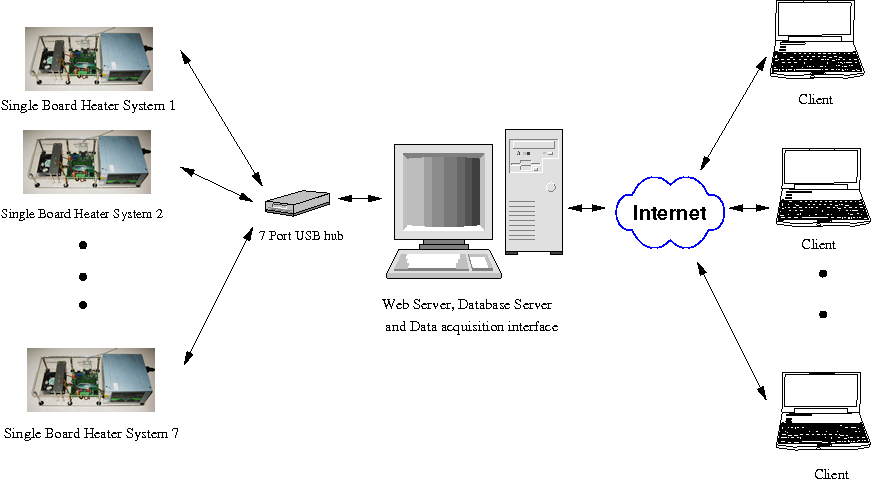
\includegraphics[width=\linewidth]{IEEE-Chile/figures/vlab-arch}
\caption{Virtual control lab hardware architecture}
\label{fig:hw-arch}
\end{figure}

\subsection{Hardware}
The architecture of the virtual single-board heater system lab as
shown in Figure \ref{fig:hw-arch} involves 7 single-board heater
systems connected to the server via a 7-port USB hub. The server
computer is connected to a high speed internetwork and has enough
processing capability to host data acquisition, database, and web
servers. The internetwork connected client computer needs only the
Java runtime engine and Scilab installation.  

A similar architecture but replacing Java with python and with 15 units connected to the server via two 7-port hubs has been successfully tested on intranet for the undergraduate Process Control course and the graduate Digital Control
and Embedded systems courses conducted at IIT Bombay as well as few workshops over the internet. Currently, this architecture is integrated with a cameras on each SBHS to facilitate live video streaming. This facility will be extended to all the units in future. This gives the user a feel of remote hands-on. Work on this camera facility is in progress.


\subsection{Software}
The current software architecture of this virtual control lab is shown
in Figure \ref{fig:detail-arch}. The server computer runs on Ubuntu
Linux 10.04 OS. It hosts a LAMP (Linux-Apache-MySQL-PHP) server. The
MySQL-based database server has the details of all the registered
users, their slot details, authentication keys to allow remote access,
etc. It also hosts a PHP based web server shown in Figure
\ref{fig:sbhs-website} that has pages for registration, login and slot
booking \cite{vl010}.  For communication with the device, Django - a Python based web framework is used on the Server side. On the client end has control
algorithms running in Scilab and communicates over the Internet
through the python client.

\begin{figure}
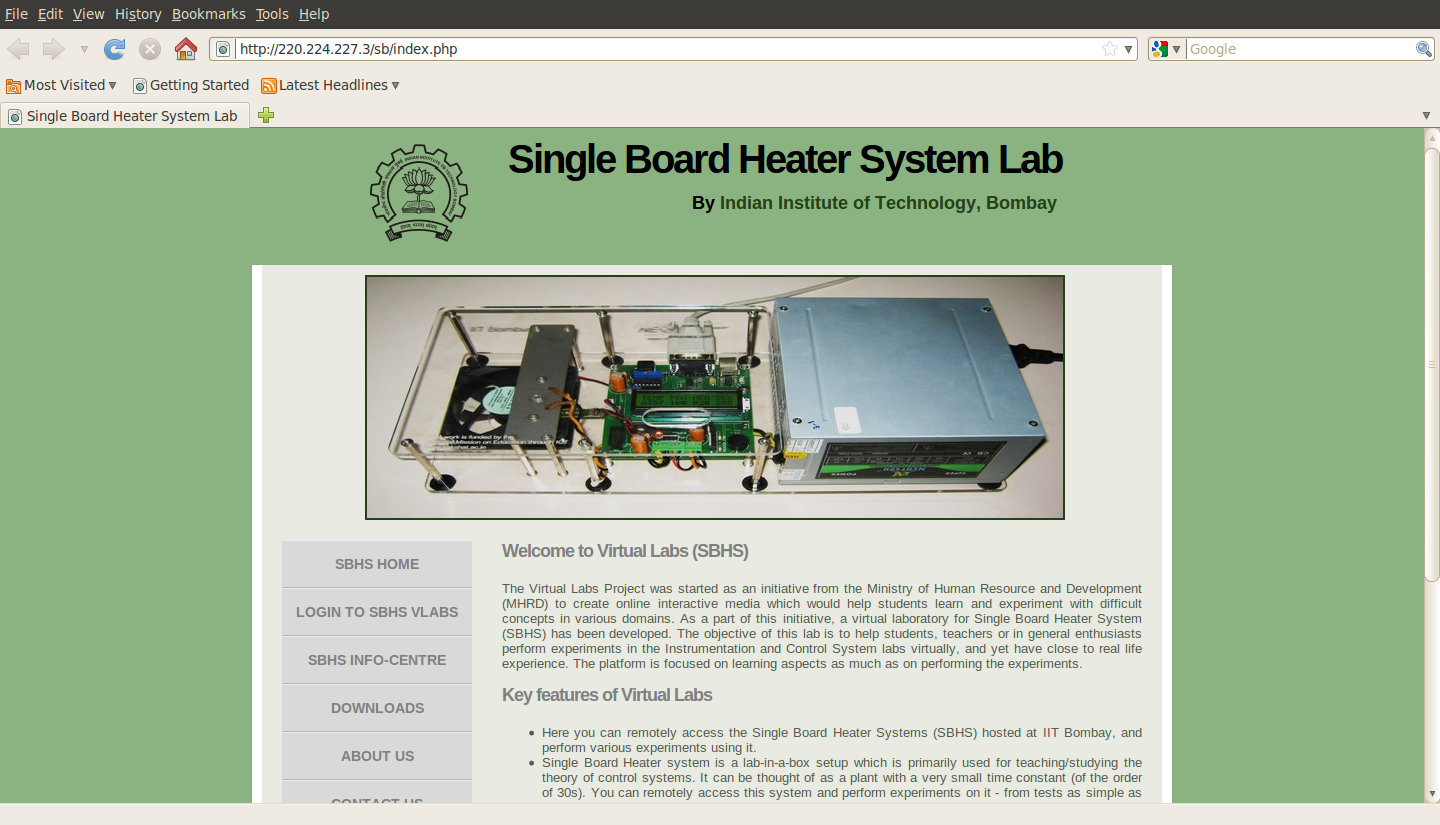
\includegraphics[width=\linewidth]{IEEE-Chile/figures/webpage}
\caption{Home page of SBHS V Labs}
\label{fig:sbhs-website}
\end{figure}
The steps to be performed before and during each experiment are explained next.

\begin{figure}
\centering
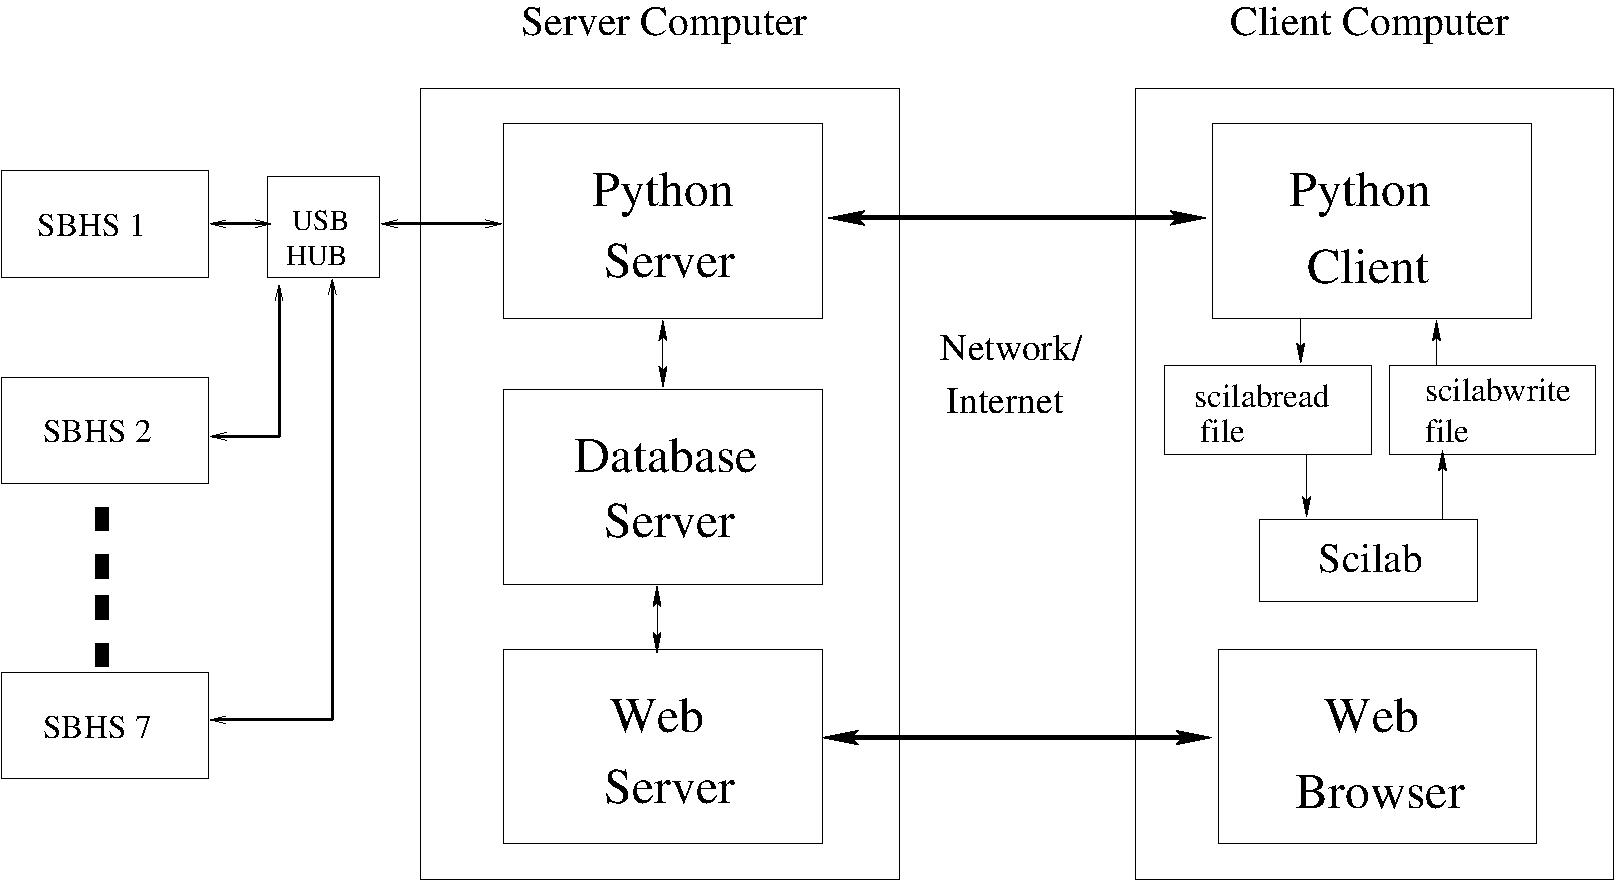
\includegraphics[width=\linewidth]{IEEE-Chile/figures/blk-dig.pdf}
\caption{Current Architecture of SBHS Virtual Labs}
\label{fig:detail-arch}
\end{figure}



\subsubsection{Registration}
A client willing to perform the experiments needs to register with us
by entering the personal details on the Registration page. This sends
an account activation link to the client’s mailbox. Upon clicking the
link, the account gets activated.
\subsubsection {Slot booking} The client can now login and book slots
to perform the experiments. Each slot lasts for an hour with 55
minutes for experimentation and 5 mins for resetting the setup. A
client can book up to 2 slots, per day, in advance. Besides this, if
the current slot is empty, it can be booked as a free slot. For each
slot being booked, the client gets a port number and an access
key. The interface depicting this is shown in Figure
\ref{fig:slot-booking}.
\begin{figure}
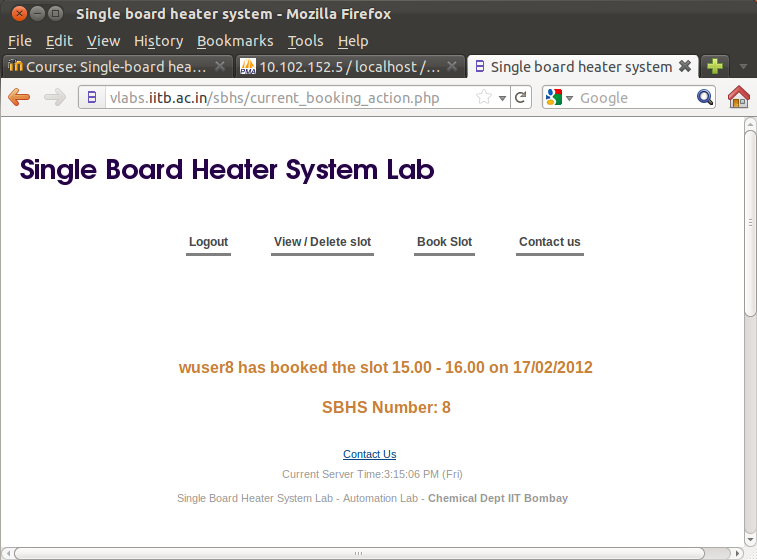
\includegraphics[width=\linewidth]{IEEE-Chile/figures/slot-book.png}
\caption{Screenshot of Slot Booking Page}
\label{fig:slot-booking}
\end{figure}
\subsubsection {Port number} In order to maintain consistency in
performing the experiments, each client is alloted the same setup
every time s/he requests for the slot. To facilitate this, each setup
has been alloted a machine I.D. For example, if the machine I.D. of
the unit is 5, it is displayed as {\tt SBHS Number: 5}. This
eliminates time and effort spent in plant modelling, each time, due to
change in the setup.

\subsubsection { Starting the Python client} On windows, after installing python, it will not be readily recognized by the OS. To make windows interpret python as a command, do the following steps.
\begin{enumerate}
\item Right click on My Computer and click on properties
\item Click on the Advanced tab.Now click on the Environment Variables button
In the system variable section, locate and click on “path”.
\item Click the edit button below it. You should see a “Edit system variable” window.
\item In the “Variable value” field, take the cursor to the last.
Type a semicolon and type C:$\backslash$Python27
\end{enumerate}
The experiment folder has a run.bat file, settings.txt file and a sbhsclient.py file. Open the settings.txt file and make the required changes. Beware not to make any unneccesary changes to this file. The example settings are anyways given in the end of this file. Linux users should bypass the terminal proxy settings, if any, by executing the command {\tt export http\_proxy=''}. Be informed that this is just a temporay disable of proxy and it should be done everytime you open a fresh terminal. Windows users simply double click on the run.bat file. It will open up a command prompt. Linux users instead of executing the run.bat file will type the following command on the terminal {\tt python sbhsclient.py}. This activity will ask you for the username and password. If the settings are not proper in the settings.txt file, you will get a {\tt Connection error message}. Contact the system administrator of your network to get the correct values of the parameters. Once you are done typing your username and password, you will get a Login Successfull message. In case if you are logging in at a time other that your booked slot, it will tell you that No slot is found. Else, it will notify that you have booked a slot and can now run the scilab code. It will also create {\tt scilabread.sce, scilabwrite.sce} and a log file in the experiment folder. The log file name will be in the format {\tt date\_month\_year\_hrs\_mins\_seconds.txt}. This unique file name will help you track the log file of you choice in the future. 
\begin{figure}
  \centering
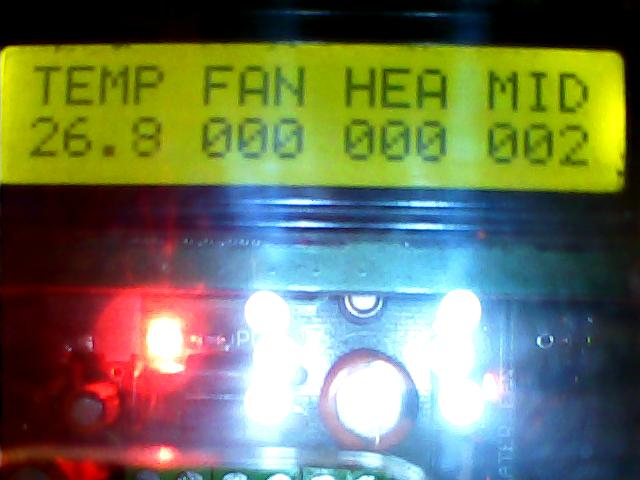
\includegraphics[width=0.7\linewidth]{IEEE-Chile/figures/display.jpg}
\caption{Screenshot of Video Stream}
\label{video}
\end{figure}
\subsubsection { Video streaming} At present, the facility to provide video streaming for all users is in progress. The video
streaming of the capture display will be something as shown in Figure \ref{video}. The clients with lesser bandwidth will have an option to refrain from video streaming. This facility will be available for logged in users on the website.

\subsubsection { Executing the Scilab code} The client needs to
download the scilab code from the SBHS home page. This is available
under {\tt Downloads}. Various other experiments are also available on {\tt fossee.in/moodle} The client can modify this code to implement
his/her own algorithm. S/he should not edit the part of the code which
is used for communicating with python. This part is clearly marked in
the code. Refer the chapter specific to which experiment you want to run. It will explain you which codes and in what order they should be executed.

\subsubsection { File handling} This subsection explains the
significance of scilabread and scilabwrite files. During the
experiment, the client writes heater and fan inputs to the
scilabwrite.sce file. These values are read by the Python client. It writes iteration and client departure time stamp and send it over the network. Python server at the other end reads these values, puts a server arrival time stamp and gives them to the SBHS through its data acquisition
interface. After feeding the values, it reads the temperature of the
heated plate, puts a server departure time stamp and sends it to the Python client. The Python client puts a client arrival time stamp and then writes all these values i.e. heater, fan and temperature along with the
timestamps to the scilabread.sce file. Scilab client reads the latest
temperature value and does the calculation of heater and fan inputs in
accordance to the logic developed for the experiment. The live data
streaming involves heater and fan inputs being sent by the client and
temperature response in turn being sent by the server. The timestamp accompanying the data could be used for real-time
control of the setup.

\subsubsection { Concluding the experiment} Once the client is done
with the experiment, s/he can use the log file created in the experiment folder for analysis purpose. If you happen to lose the log file, you can download it from the website, after you login, by clicking on {\tt Download} link.
%\end{enumerate}

\subsection{Other Implementation Issues}
%\begin{enumerate}
\subsubsection { Mapping of machine id with the USB port number}
Whenever a SBHS unit is plugged in to a USB port, the dev id (/dev/ttyUSB*) assigned to it by OS is different. A script is run which creates a table of the mapping between the machine I.D. and the USB dev id. This is done to ensure that the client gets the same machine I.D. i.e. the same SBHS each time. 

\subsubsection { Auto log off problem}
In some ISPs, the network gets disconnected if it is inactive for some time. To handle this situation, we are running a shell script which checks for internet connectivity by pingging google periodically. If the network is down then it will try to reconnect.  


%\end{enumerate}


\subsection{Support}
The SBHS support activities are being funded by National Mission on Education through Information and Communication Technology \cite{kmm010}.  The major support activities include conducting workshops in several colleges across the country, active discussion through Fossee moodle and spoken tutorials for self-learning.

\subsubsection{Workshops}
The SBHS team has been conducting workshops to popularise the utility of SBHS.  The course content is around local and remote access of the SBHS. More than 50 college teachers from several Engineering colleges of the country have attended the workshops and have started using the setup for the relevant courses running in their colleges.

\subsubsection{Fossee moodle}


Fossee moodle is a web interface that allows discussions, post queries, upload files, upload grades, etc.  Also, there is a facility to provide e-mail notification whenever there is a post on the course website. Thus, such an interface allows to address common problems of many users at the same time. It also provides a platform for the users at different locations to share their experiences during the experiments.  The codes and manuals for about 8 experiments are available at \cite{moodle}.


\begin{figure}
\centering
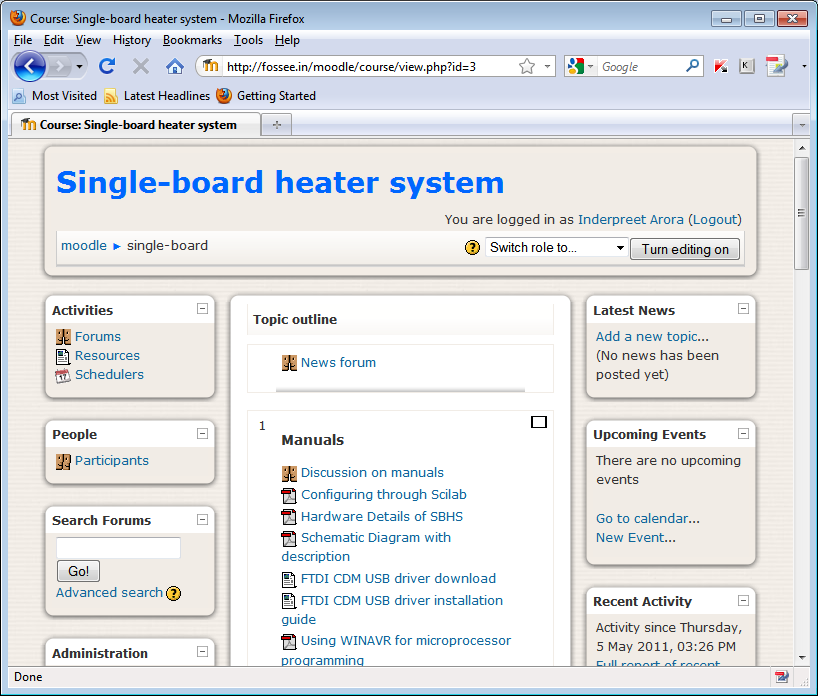
\includegraphics[width=0.75\linewidth]{IEEE-Chile/figures/fossee-2}
\caption{Fossee moodle webpage to support SBHS activities}
\label{fig:fossee-sup}
\end{figure}



\subsubsection{Spoken tutorials}
A Spoken tutorial is a screen capture along with the audio that could be used to teach any computer application.  Currently, the spoken tutorials for various Free and Open source softwares are available in different Indian languages at \cite{spoken-sci}.  The scripts and tutorials for SBHS are in pipeline.




\section{Experiments}
\label{sec:expts}
About 10 experiments have been performed using SBHS locally while about 5 of them through remote access.  The open loop experiments are not affected much with a moderate amount of network traffic.  However, key learning is while implementing the control algorithms and observing the effect of network delay.  The results of a few experiments are presented next.

\subsection{Identification using step response data}
As reported in \cite{ia010}, the step test experiment has been conducted by giving 2 step changes of 5 PWM units each and allowing the temperature profile to stabilize each time.  The process model is then identified using this step response data
\cite{karl95,seborg04}. Notably, the remotely performed experiments reported in this paper are done on the same unit reported in \cite{ia010}.  

For the given two step changes, we got the following models \cite{ia010}:
\begin{align*}
G_1 &= \frac{0.62}{44s + 1}e^{-10s}, \ 
G_2 = \frac{0.65}{50s + 1}e^{-10s}
\end{align*}


\subsection{PID control}
The efficacy of the PID controller, in discrete form, is explored next.
\begin{align}
u(t) = K\left[e(t) + \frac{1}{\tau_i} \int_0^t e(t)\,dt + \tau_d
  \frac{de(t)}{dt}\right] 
\end{align}

With the data acquired after every $T_s$ seconds, the integral and derivative terms can be approximated as,
\begin{align}
\int_0^t e(t)\,dt & \approx T_s \sum_{i=0}^{t} e(i) \\ 
\frac{de(t)}{dt} & \approx \frac{e(t) - e(t-1)}{T_s} 
 \end{align}

Using the reaction curve method for the models of the two step response experiments stated earlier,  we arrive at the following values: 

\begin{align*}
L_1 = 10, \tau_1 &= 90, K_1 = 0.62 \\
L_2 = 10, \tau_2 &= 105,K_2 = 0.65
\end{align*}


\subsubsection{Local implementation}
This experiment implements the PID controller locally i.e. the user has a unit connected to his/her computer.

Using the first set and the relations $K_p=0.9/RL$,
$\tau_i=3L$, we arrive at:
\begin{align*}
u & = \text{ubias} + K_p\left[\text{et} +
  \frac{\text{eti*Ts}}{\tau_i}\right] \\ 
K_p & = 13.06, \tau_i = 30 \\
\text{et} & = \text{setpoint - temp, eti = eti + et}
\end{align*}
 
where eti is the accumulated error.  The response for this controller
is depicted in Fig. \ref{fig:pid-2}.  This has been described in greater detail in \cite{ia010}.

\begin{figure}
\hspace{-0.2in}
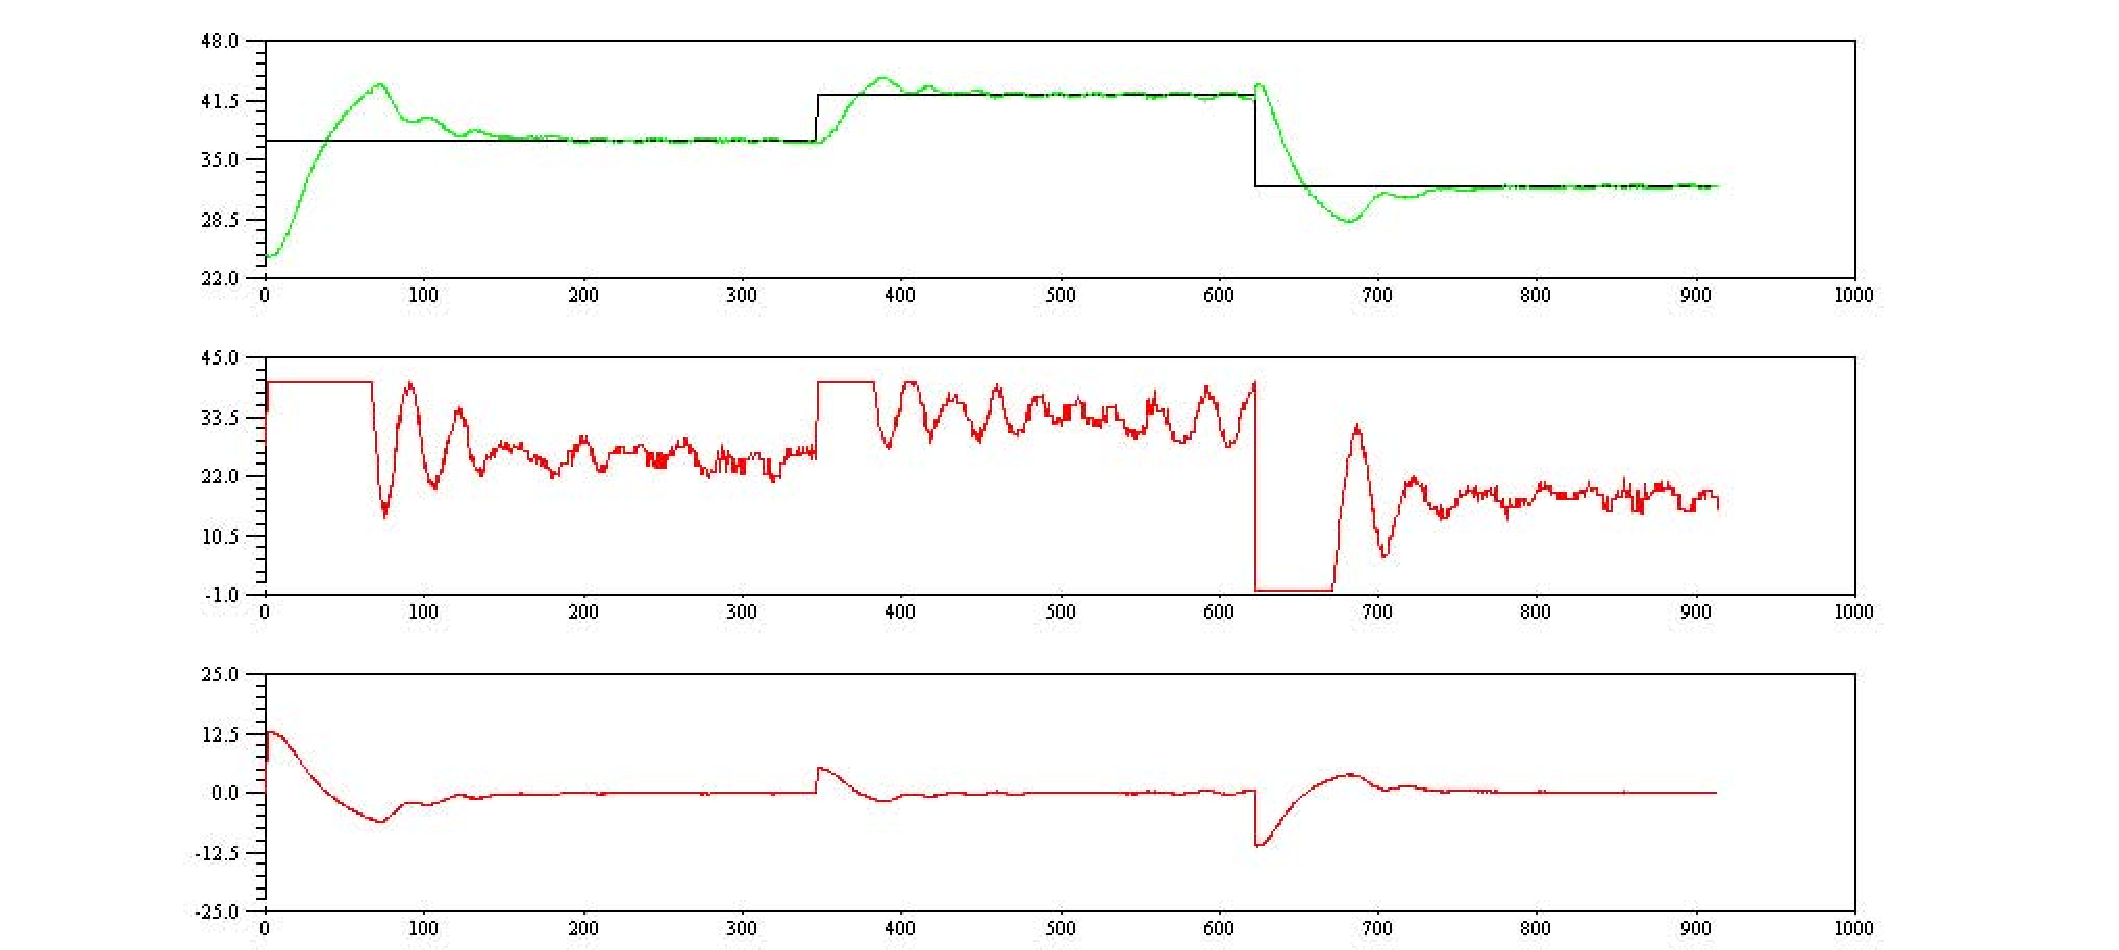
\includegraphics[width=1.2\linewidth]{figures/pi-1}
\caption{Local PI controller implementation: temperature, heater duty,
  error} 
\label{fig:pid-2}
\end{figure}


\subsubsection{Over intranetwork}
The control effort for the same implementation but over network is found to be oscillatory.  The experimental result is depicted in figure \ref{fig:pidosc}.  Next, we re-tune the controller to get better results.

\begin{figure}
\hspace{-0.2in}
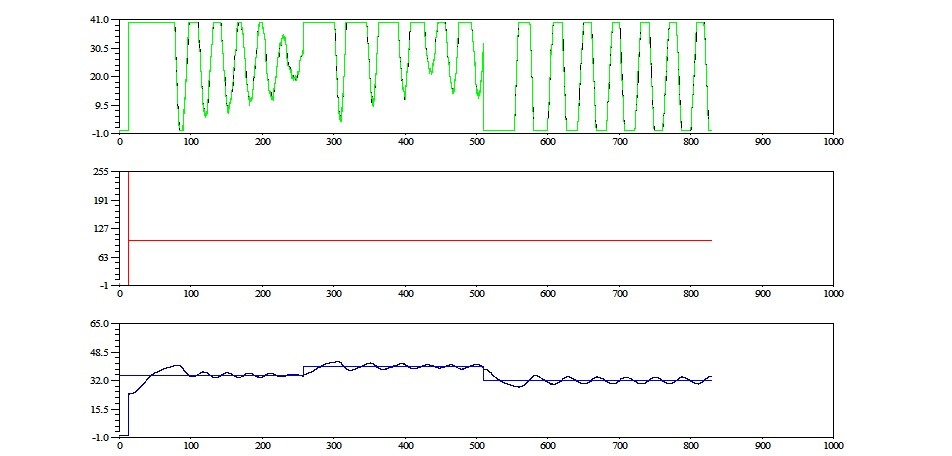
\includegraphics[width=1.2\linewidth]{figures/pidc_intra_osc}
\caption{PID control with local PID tuning parameters and remote
  implementation: heater duty, fan speed, temperature}
\label{fig:pidosc}
\end{figure}

%Tightly tuned real time PID control
In order to implement an acceptable control algorithm, we either need to compensate for time delay or tightly tune the controller.  The source of time delay is network traffic.  With multiple applications running on the same machine and the sampling done every 0.4 s, a small amount of time is also spent in reading from and writing to a file at both the ends.

We implemented the controller with the tuning parameters, $K_p = 2$, and $\tau_i = 50$.  The real implementation results are shown in figure \ref{fig:pidctun}.  The tracking is found to be satisfactory.

\begin{figure}
\hspace{-0.2in}
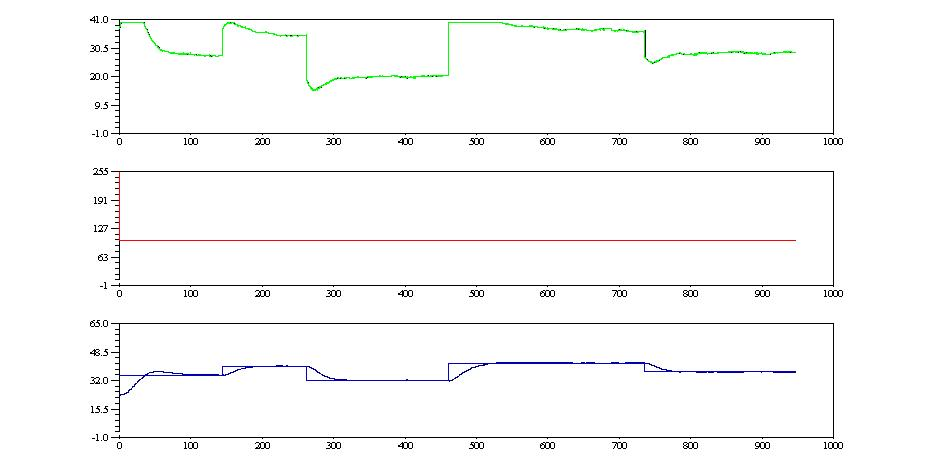
\includegraphics[width=1.2\linewidth]{figures/pidc_intra}
\caption{Tuned PID controller and remote implementation: heater duty,
  fan speed, temperature}
\label{fig:pidctun}
\end{figure}

The possibility of real-time control using a disturbance observer
\cite{kempf96,jones07} is being explored. 

\subsection{Two Degrees of freedom Controller}
\label{2dof}
A Two Degrees of freedom Controller (2-DOF) strategy \cite{kmm07} was
implemented remotely on SBHS through virtual lab. A block diagram for
the same is as shown in the Figure \ref{2doffig}. After performing the
step test, the second order transfer funtion obtained was  
\begin{align*}
G(s)&=\frac {1.029}{(71.16s+1)(s+1)}
\end{align*}
with time constant $\tau_1 = 71.16 sec$, $\tau_2 = 1 sec$  and gain $K=1.029$.
%
\begin{figure}
\centering
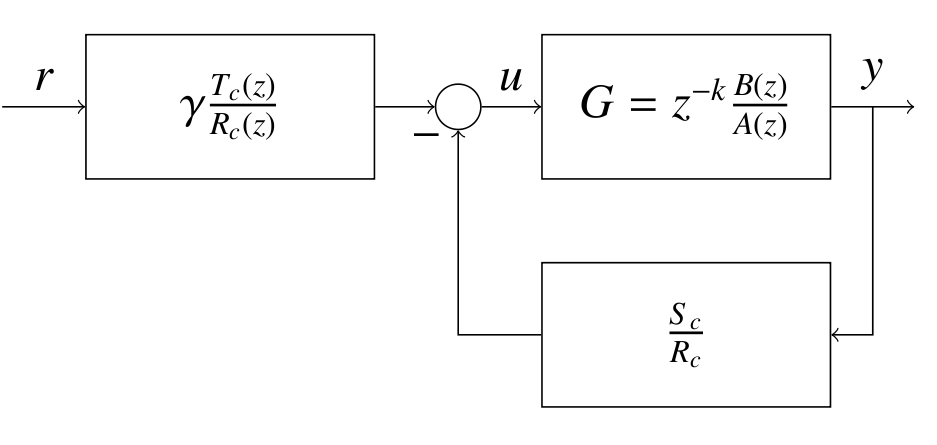
\includegraphics[width=\linewidth]{figures/2dof.png}
\caption{Two Degrees of freedom Controller structure}
\label{2doffig}
\end{figure}
%
For rise time = 20 seconds and Overshoot of 5\%, the various
controller parameters obtained are
\begin{align*}
R_c &=  0.0143941 -  0.0345042z^{-1}  + \\&0.0265766z^{-2} - 0.0064665z^{-3}  \\
S_c &=  0.0045849  - 0.0045528z^{-1}\\
T_c &= 1.  - 0.9929982z^{-1}\\
\gamma &= 0.004589
\end{align*}
The response of the controller implented on SBHS virtually is as shown
in the Figure \ref{2dofresp}.


\begin{figure}
\hspace{-0.2in}
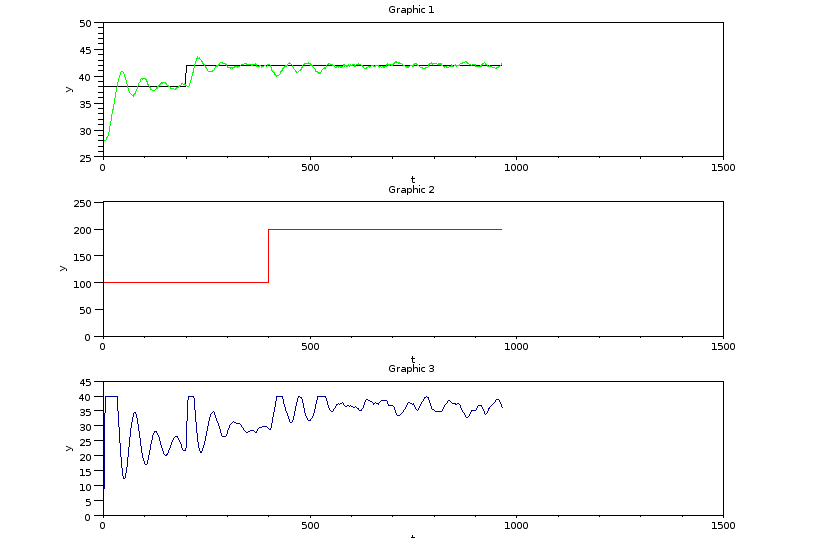
\includegraphics[width=1.2\linewidth]
{figures/twodof_disturbance_intranet.png}
\caption{2-DOF controller implementation: temperature, fan speed,
  heater duty}
\label{2dofresp}
\end{figure}


\subsection{Identification of PID parameters using Relay Feedback Technique}
Relay feedback auto-tuning method developed by Astrom and Huggland is
one of the simplest and most popular auto-tuning technique for process
control applications\cite{karl84}. In this method, a simple
experimental test is used to determine ultimate gain and ultimate
period. 

\begin{figure}
\hspace{-0.2in}
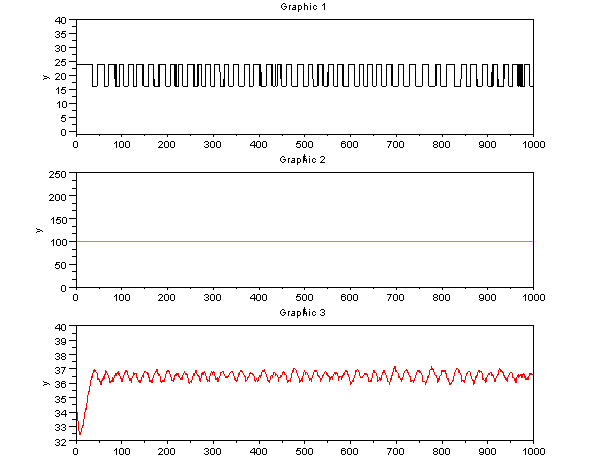
\includegraphics[width=1.2\linewidth]{figures/relay.png}
\caption{Relay feedback implementation: heater duty, fan speed,
  temperature} 
\label{relayresp}
\end{figure}

\begin{figure}
\centering
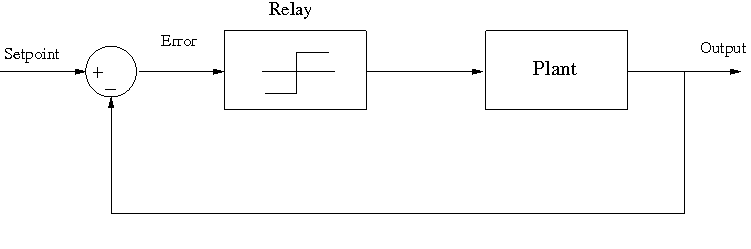
\includegraphics[width=\linewidth]{figures/relay1.png}
\caption{Conventional relay feedback system}
\label{relaysys}
\end{figure}

A feedback controller is temporarily repalced by an On-Off controller (or a relay) as shown in the Figure \ref{relaysys}. When the control loop is closed, the control variable exhibits a sustained oscillations which is a property of On-Off controller.

Relay feedback method has been implemented on Single board heater system using virtual labs.


From the Figure \ref{relayresp}, we can observe the sustained
oscillations in temperature. 
Using the expressions derived by \cite{karl84}, the following
parameters are obtained:
The Ultimate period Pu = 25 seconds.
The Ultimate gain Kc = 5.66.  The                    
PID parameters are then calculated from Ziegler-Nichols controller
settings shown in Table \ref{2ndmtd}. 
\begin{table}
\begin{center}
\renewcommand{\arraystretch}{1.5}
\begin{tabular}{|c|r|r|r|}\hline
Type of
controller & $K_{c}$ & $\tau_i$ & $\tau_d$ \\ \hline
$P$ & $0.5K_{cu}$ & $\infty$ & 0 \\ \hline
$PI$ & $0.45K_{cu}$ & $ 0.8334P_{u}$ & 0 \\\hline
$PID$ & $0.6K_{cu}$ & $0.5P_{u}$ & $0.125P_{u}$ \\ \hline
\end{tabular}
\caption{Ziegler-Nichols Controller Settings based on the Continous Cycling Method}
\label{2ndmtd}
\end{center}
\end{table}%
The PID parameters are obtained as
$K_{c}$ = 3.3939394,
$\tau_i$ = 12.5, and 
$\tau_d$ = 3.125.


           

%\section{Real-time control}

\section{Conclusions}
In this work, we presented a virtual laboratory that is based entirely
on free and open source software.  This solution is scalable as it is
affordable.  It is also in line with the objectives of the funding
agency \cite{kmm010} that aims to promote open educational resources.

The solution presented in this work allows about 100,000 hours of
experimentation time in a year with one or at most two server PCs
working with about 20 SBHS.  Thus, this configuration has the
potential to cater to the million students who enroll in engineering
colleges in India every year.

The main shortcomings of the approach followed in this work are due to
the delay introduced in the loop by the Internet.  We are at present
studying the efficacy of delay observers \cite{kempf96,jones07} to
address this issue.


%The paper explains a low cost, scalable, virtual control laboratory.  This cost effective solution can be extended to any type of setup thereby giving more hands-on experimentation to the students.  Even the colleges with the lack of infrastructure can train their students using this approach.  This web based solution has a potential to bridge the gap between theory and practice.  




\bibliography{ref1}

% conference papers do not normally have an appendix


% use section* for acknowledgement
\section*{Acknowledgments}
The authors gratefully acknowledge the funding support from the
National Mission on Education through Information and Communication
Technologies \cite{kmm010}.

The authors would like to thank Ankit Bahuguna, Harsh Yadav, Piyush
Joshi, Kushal Thakkar, Swanand Kulkarni, Aditya Sengupta, Sushanth
Poojary, Tanuj Bhojwani and Sitesh Patel for their inputs for a few
software modules.  

\end{document}
